\documentclass{article}
\usepackage{graphicx} % For including images
\usepackage{titling}  % For custom title page
\usepackage{circuitikz}
\usepackage{amsmath}
\usepackage{amssymb}
\usepackage{booktabs,tabu}
\usepackage[all, cmtip]{xy}
\newcommand{\ohm}{\Omega}
% Set up title and author
\title{Experiment 1: Basic Filter Design}
\author{Samyak Sheersh,Souhardya Bose,Aryam Shankar}
\date{20 August 2024}
\newcommand{\subtitle}[1]{%
  \posttitle{%
    \par\end{center}
    \begin{center}\large#1\end{center}
    \vskip0.5em}%
}

\begin{document}

% Custom title page
\begin{titlepage}
    \centering
    
\includegraphics[width=0.2\textwidth]{KGP_logo.png}\par\vspace{1cm}
    {\scshape\LARGE Department of Electronics and Electrical Communication Engineering, IIT Kharagpur\par}
    \vspace{1cm}
    {\huge\bfseries Experiment 5: FM Demodulation\par}
    \vspace{1.5cm}
    {\Large\itshape Samyak Sheersh,Souhardya Bose,Aryam Shankar\par}
    \vfill
    % Identifying information at the bottom
    {\large Roll Numbers: 22EC30045, 21EE10097, 22EC3FP37\par}
    {\large Group Number: 12\par}
    \vfill
    {\large 15 October 2024\par}
\end{titlepage}


\section{Introduction}
We use IC 565 to perform frequency demodulation of an FM signal and observe the output waveforms in the time and frequency domains. We also observe the waveforms on the DSO and perform FFT analysis.
\section{Objectives}
\subsection{Task 1}
Without providing the FM Input, check the internal VCO Output Waveform of the PLL IC on the oscilloscope. Adjust the potentiometer at R1, to set the frequency of VCO output to 10 KHz. (10 KHz is the carrier frequency chosen for modulation)
\subsection{Task 2}
Provide the FM Input at pin 2 of PLL IC and observe the PLL O/p waveform at pin no 7 of IC. An additional low pass filter can be added to the circuit to eliminate frequency components other than modulating signal frequency 1 KHz from PLL output.
\subsection{Task 3}
Apply a square wave message m(t) to the point Vc of the circuit and observe the frequency-modulated signal at the output pin on DSO. (Take modulating signal’s fm = 1KHz). Demodulate the FM-modulated signal to get back the square wave message signal, without using any IC, but only using standard components.
\subsection{Task 4}
Demodulate the FM-modulated sinusoidal signal to get back the sinusoidal message signal, without using any IC, but only using standard components.
\section{Instruments and Materials Used}
\begin{enumerate}
  \item RIGOL Signal Generator
  \item ScientiFIC SMO10C Digital Signal Oscilloscope
  \item +12V, -12V DC source and ground
  \item Resistors
  \item Capacitors
  \item Diodes
  \item Breadboard
  \item Connecting wires
  \item IC 565
  \item Potentiometer
\end{enumerate}

\section{Theory}
The peak deviation frequency is denoted by 
\begin{equation}
  \Delta f= f_{max}-f_c
\end{equation}
and the modulation index($m$) is given by
\begin{equation}
    m=\frac{\Delta f}{f_m}
\end{equation}
The carrier frequency without modulating the signal can be adjusted by tuning the potentiometer and is guided by the following relation
\begin{equation}
    f_c=\frac{1}{RC}
\end{equation}

The instantaneous carrier frequency after modulation is guided by the following relation(VCO)
\begin{equation}
  f_c=\frac{1}{RC}\Big[1+\frac{R}{R_c}\Big(1-\frac{V_c}{3}\Big)\Big] \ Hz
\end{equation}
where $V_c$ is the control voltage guided by a message signal connected through the resistance $R_c$ to pin 7.

\subsection{Circuit Diagram}
\begin{figure}[!ht]
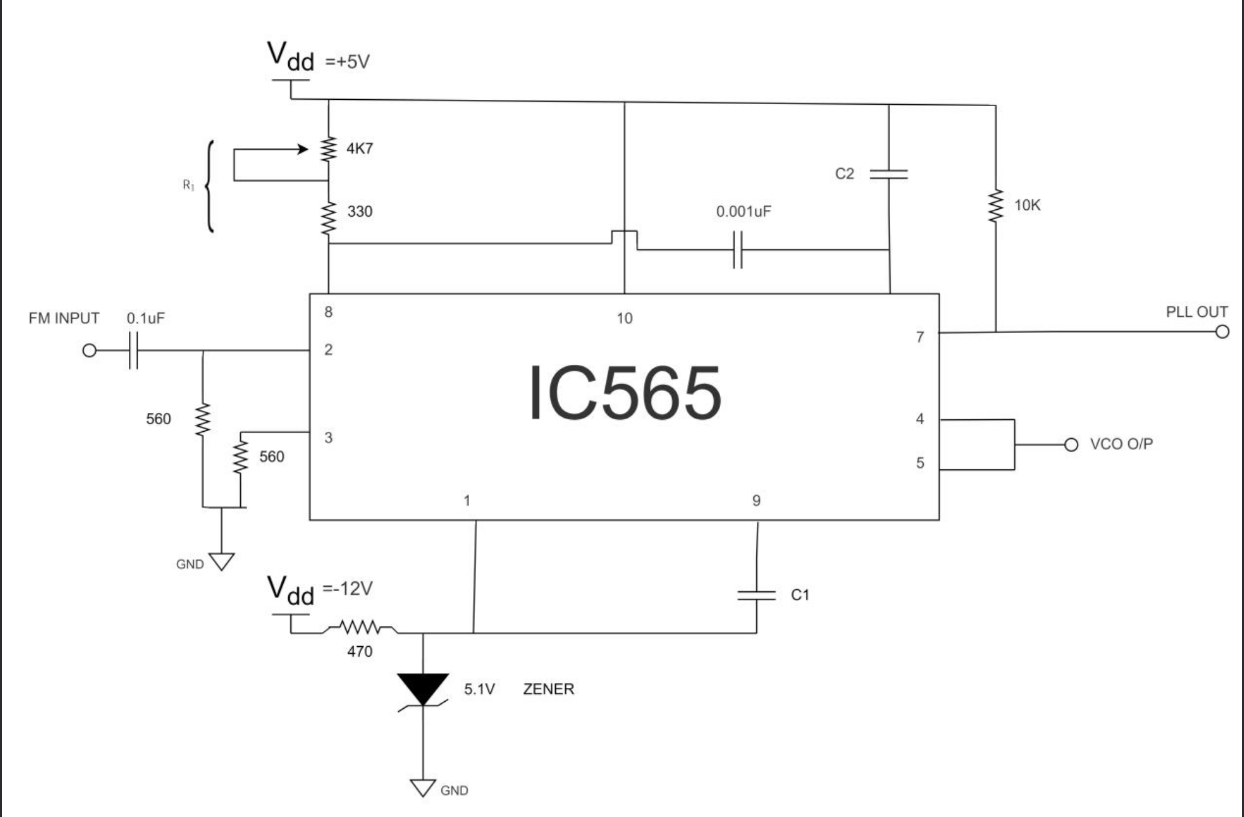
\includegraphics[width=\textwidth]{Circuit.png}
\caption{Circuit Diagram}
\label{fig:cir}
\end{figure}
\clearpage
\subsection{Calculations}
The free running frequency of VCO is $f_0 = 10 \ kHz$ (Centre Frequency)
\begin{equation}
    f_0=\frac{1}{4R_1C_1}
\end{equation}
taking $R_1=4k\Omega$, we get $C_1=6.2nF$

For the internal low-pass filter design
\begin{equation}
    f=\frac{1}{2 \pi 3.6 k\Omega C_2}
\end{equation}
Taking $C_2=0.033\mu F$, we get $f=1.3 kHz$
\section{Observations}
\subsection{Task 1}
\begin{figure}[!ht]
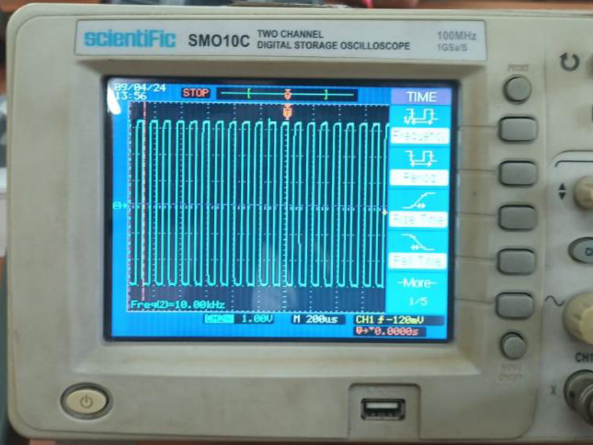
\includegraphics[width=\textwidth]{FRF.png}
\caption{DSO showing the free running frequency of the VCO at f=10kHz}
\label{fig:FRF}
\end{figure}

\subsection{Task 2}
We apply the frequency-modulated input at pin 2, and observe the demodulated PLL output waveform at pin no 7 of IC. An additional low pass filter is added to the circuit to eliminate frequency components other than modulating signal frequency 1 KHz from PLL output so that we get a cleaner demodulation.

\begin{figure}[!ht]
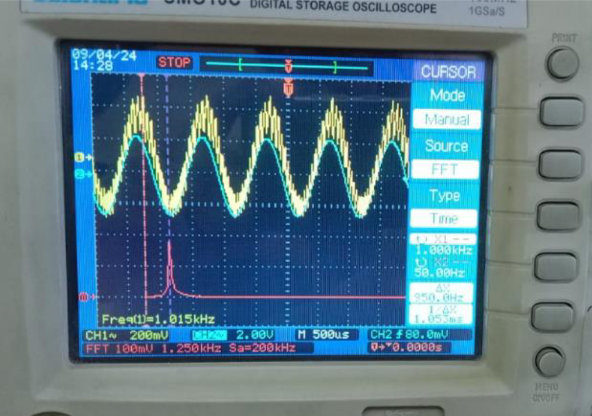
\includegraphics[width=\textwidth]{Output.png}
\caption{Demodulated output without applying the lowpass filter}
\label{fig:no_LPF}
\end{figure}

\begin{figure}[!ht]
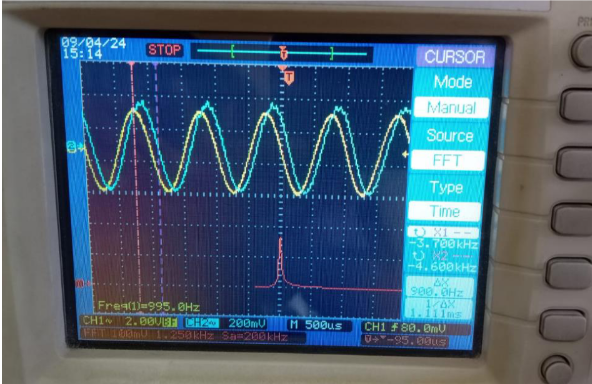
\includegraphics[width=\textwidth]{Filtered.png}
\caption{Demodulated output after applying the lowpass filter, on top of the original message signal}
\label{fig:LPFd}
\end{figure}

We observe a phase shift and the DSO showing the frequency at 995 Hz, slightly below our original signal at $f_m=1000 \ Hz$. 
\subsection{Task 3}
Here we couldn't use an IC to demodulate the signal and had to use standard components to decode a square signal. This is the circuit that we came up with:
\begin{figure}[!ht]
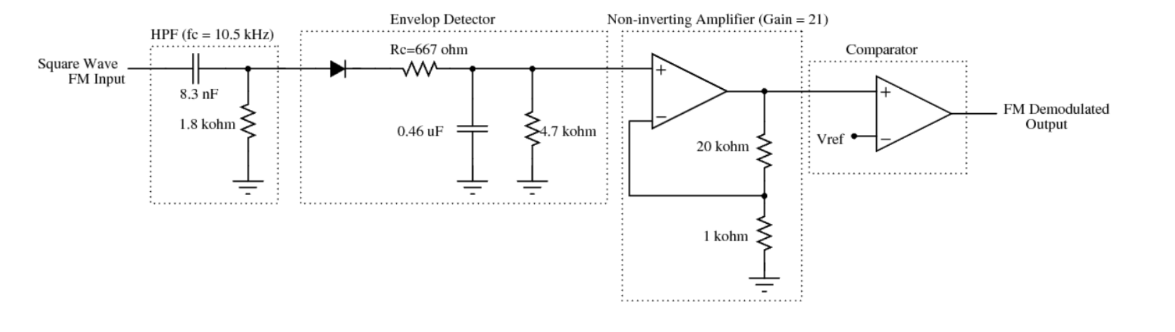
\includegraphics[width=\textwidth]{Demod_1.png}
\caption{The circuit for demodulating an FM modulated square signal input using standard components}
\label{fig:cir_1}
\end{figure}

\begin{figure}[!ht]
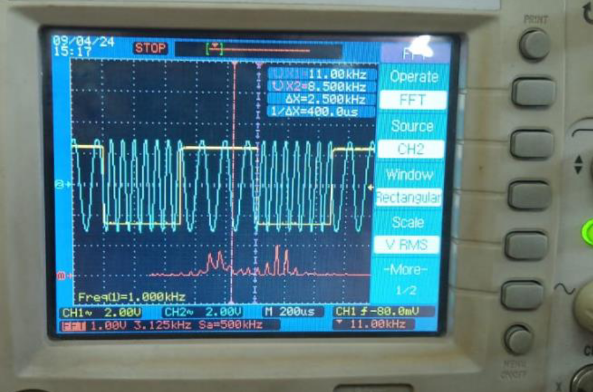
\includegraphics[width=\textwidth]{Input_sq.png}
\caption{FM Modulated Input to the circuit superimposed on top of the original square wave signal}
\label{fig:inp_sq}
\end{figure}

\begin{figure}[!ht]
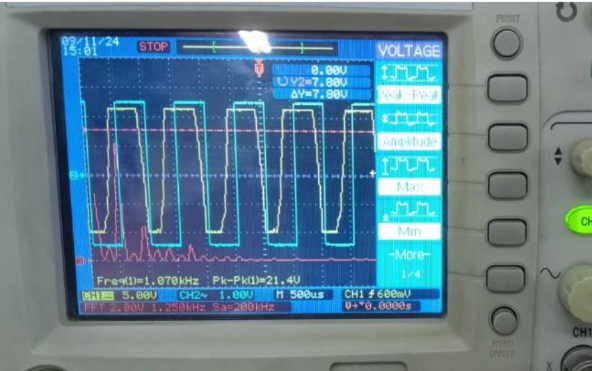
\includegraphics[width=\textwidth]{Output_sq.png}
\caption{Demodulated output of the circuit superimposed on top of the original square wave signal}
\label{fig:out_sq}
\end{figure}

From the DSO output and FFT analysis, we observe that the output frequency of the demodulated waveform is 1.07 kHz(slightly bigger than 1kHz, but acceptable). The FFT analysis, shows the proper frequency spectrum of the demodulated output waveform for a square wave.
\clearpage
\subsection{Task 4}
Here we had to design a demodulator for a sinusoidal signal without using an IC, and this is the design we came up with, which is essentially a differentiator followed by an envelope detector:
\begin{figure}[!ht]
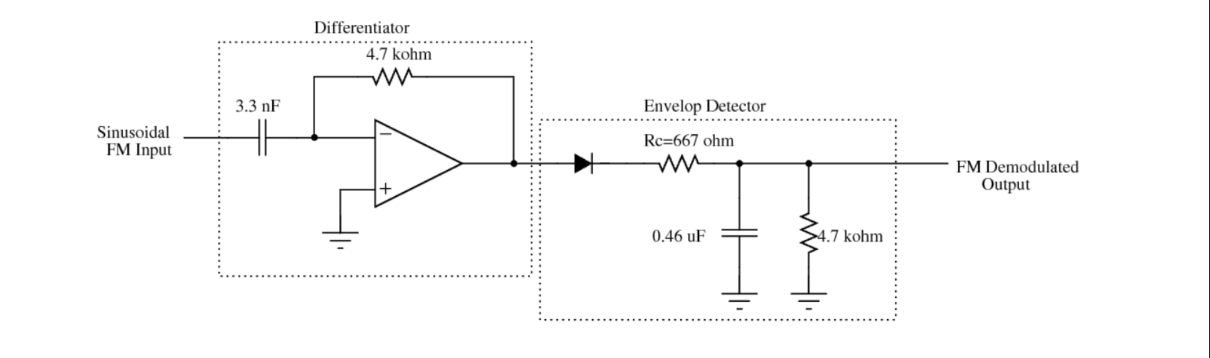
\includegraphics[width=\textwidth]{Demod_2.png}
\caption{The circuit for demodulating an FM modulated sinusoidal signal input using standard components}
\label{fig:cir_2}
\end{figure}

\begin{figure}[!ht]
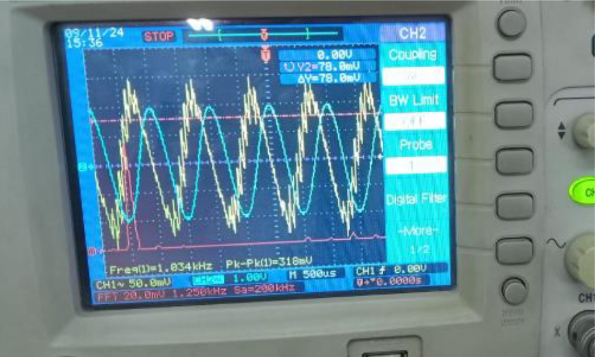
\includegraphics[width=\textwidth]{Output_sin.png}
\caption{FM demodulated signal superimposed on top of the original signal}
\label{fig:out_sin}
\end{figure}

We can again see from DSO analysis that the output frequency of the demodulated waveform is 1.034 kHz(slightly bigger than 1kHz but acceptably small error), and that the FFT is also proper for this demodulated output
\clearpage
\section{Discussion}
\subsection{Samyak Sheersh, 22EC30045}
\begin{enumerate}
  \item We observed that the frequency-modulated waveform is out of phase with the modulated input signal. We tune the potentiometer to adjust the output frequency and it provides the desired control voltage to the VCO for generating that frequency. As this bias level approaches $\frac{V_{dd}}{2}$, the phase of the output signal is reversed, and the amplitude goes through zero.
  \item We used a steep High pass filter in the case of square signal to discriminate between the lower and higher frequencies of the signal and thus apply the comparator to result it back into a square signal with 1 representing the pass frequencies which are higher than the stopped frequencies which are lowered. 
  \item We used a differentiator in the sine wave signal because when we differentiate the signal, the term varying with time(which in our case is the message signal) comes out:
    \begin{equation}
        \frac{d}{dt}A\sin(\omega(t)\cdot t +\phi_0)= \omega(t) (A\sin(\omega(t)\cdot t +\phi_0))
    \end{equation}
  and thus this acts like an Amplitude modulator, on which we apply the Envelope detector to recover the signal back. 

\end{enumerate}
\end{document}

